%----------------------------------------------------------------------------------------
%	PACKAGES AND DOCUMENT CONFIGURATIONS
%----------------------------------------------------------------------------------------
\documentclass[10pt,a4paper]{article}

% Adjusting margins to personal my need
\addtolength{\oddsidemargin}{-.5in}
\addtolength{\evensidemargin}{-.5in}
\addtolength{\textwidth}{1in}
\addtolength{\topmargin}{-.5in}
\addtolength{\textheight}{1in}

% Graphics
\usepackage{caption}
\usepackage{subcaption}
\usepackage{floatrow}
\usepackage{graphicx}
\usepackage{float}
\usepackage{adjustbox}

\graphicspath{{figures/}}

% Math
\usepackage{amssymb}
\usepackage{amsmath} % Required for some math elements 

% Other
\usepackage{algorithmic}
\usepackage{array}
\usepackage{lipsum}
\usepackage{hyperref}
\usepackage{dirtytalk}
\usepackage{enumitem}




%----------------------------------------------------------------------------------------
%	MAIN PART
%----------------------------------------------------------------------------------------
\begin{document}

\newcolumntype{M}[1]{>{\centering\arraybackslash}m{#1}} %Used for tables e.g., in section 5.3
\floatsetup[table]{capposition=top, captionskip=2pt} %Used with floatrow package to place table captions on top of the table instead of below

\title{Project Plan} % Title
\author{Company 1 - TDDC88}
\date{} % Date for the report
\maketitle % Inserts the title, author and date




\begin{table}
\centering
\begin{tabular}{||c c c c c||} 
\hline
Version & Author & Updates & Reviewed by & Date \\ [0.5ex] 
\hline\hline
0.1 & \begin{tabular}{@{}l@{}} A. Nilsson \&\\S. Gharedaghi\end{tabular} 
& Initial version & D. Ma & 2021-09-16 \\ 
\hline
0.2 & \begin{tabular}{@{}l@{}} A. Nilsson \&\\S. Gharedaghi\end{tabular}
& 
\begin{tabular}{@{}l@{}} Updated from feedback\\and added SOP\&Risks\end{tabular}
& D. Ma & 2021-10-15 \\
\hline
0.3 & D. Ma  & Minor fixes in section 4 & E. Sköld & 2021-11-02 \\
\hline
0.3 & S. Gharedaghi  & Adding roles description in section 4 & D. Ma & 2021-11-06 \\
\hline
0.4 & D. Ma  & 
\begin{tabular}{@{}l@{}} Developed section 5.1, 5.3,\\ added subsection 5.5 \end{tabular}
 & E. Sköld & 2021-11-08 \\
\hline
0.5 & D. Ma  & Developed section 5.1-5.3 & A. Nilsson & 2021-11-17 \\
\hline
0.6 & A. Nilsson  & \begin{tabular}{@{}l@{}} Added risk process \\ in chapter 6, updated CFT \\ description in section 4.2\end{tabular}  & D. Ma & 2021-11-19 \\
\hline
0.7 & F. Dolk  & \begin{tabular}{@{}l@{}} Added requirements process in 5.4 \\ \end{tabular}  & D. Ma & 2021-11-20 \\
\hline
0.8 & E. Sköld  & \begin{tabular}{@{}l@{}} Updated section 4 with role changes \\ \end{tabular}  & D. Ma & 2021-11-24 \\
\hline
\end{tabular}
\end{table}



%----------------------------------------------------------------------------------------
%	Table of Content
%----------------------------------------------------------------------------------------
\setcounter{tocdepth}{2}
\tableofcontents


\clearpage

%----------------------------------------------------------------------------------------
%	Main Part
%----------------------------------------------------------------------------------------
\section{Introduction}
\label{sec:introduction}

This education plan is written with the purpose of clarifying what knowledge areas are important in order to succeed with the given assignment, what expertise is existent in the company from the onset, and what knowledge that has to be required. The education plan will also document what the company leadership has done in order to provide each member with the necessary knowledge. This document will be continually updated with input from the department managers and team leaders. 

\section{Scope}

\label{sec:scope}

The following Work-Breakdown-Structure (WBS) shows an overview of what the project aims to fulfill and how we will achieve it.
\begin{figure}[ht]
    \centering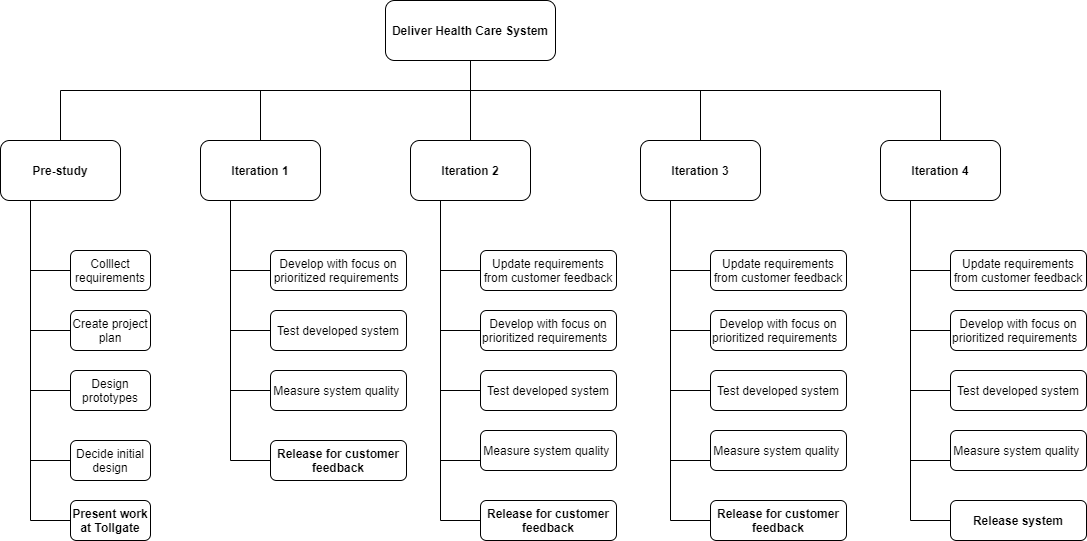
\includegraphics[width=1 \linewidth]{figures/wbs_tddc88.png}
    \caption{Work Breakdown Structure}
    \label{fig:example1}
\end{figure}


\section{Delivery to customer}
The system is going to be developed in four iterations that all end with a delivery to the customer. After each delivery we seek feedback and thoughts from the customer to get an idea in what direction we should continue with the project. The feedback will help us develop new or update our existing requirements. After the fourth iteration we will present the system at VSSE'21 - Valla Software and System Expo the 16th of December 2021.  
%\section{Company-wide}
\section{Organization and employees}
\label{sec:companywide}

The company is divided into two departments, Product \& Sales (P\&S) and Research \& Development (R\&D). The focus of the P\&S department is mainly customer contact, requirements, and testing. The R\&D department mainly focuses on topics regarding design and implementation. From these teams, we have created cross-functional teams with specific tasks. These teams have developed during the project to focus on different tasks as the project's needs have changed, see more under \ref{sec:companywide:subsection:cft} %expand this part 
\subsection{Roles}
\begin{figure}[ht]
    \centering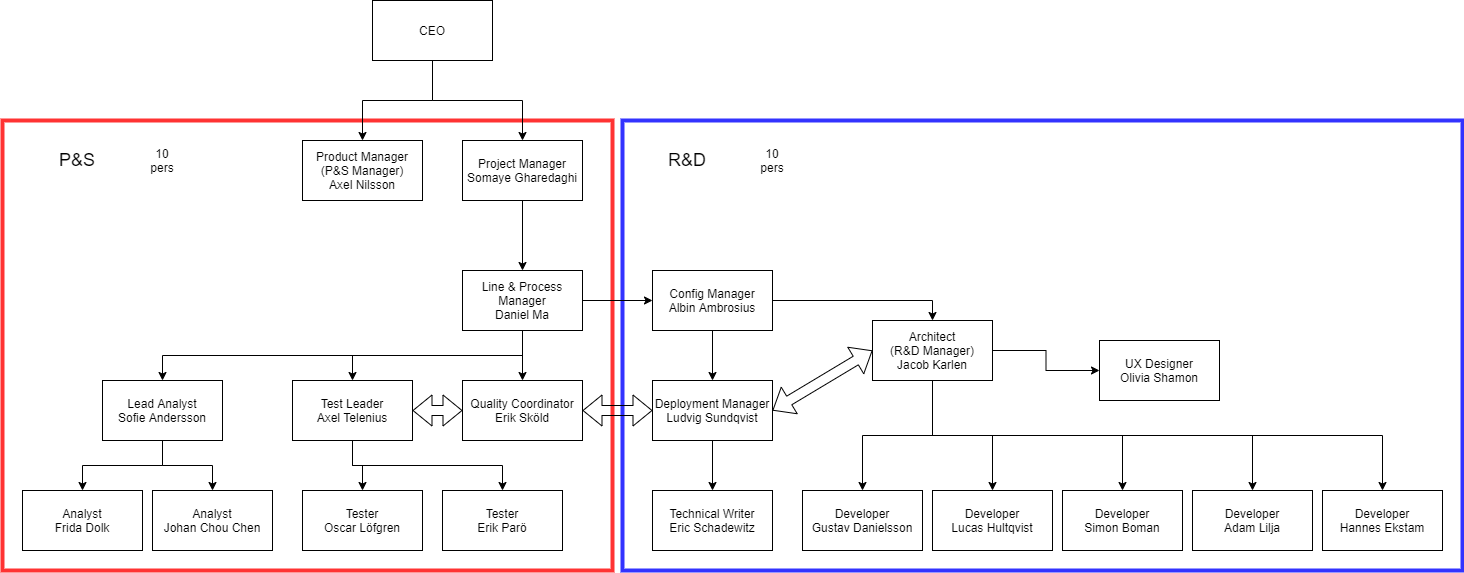
\includegraphics[width=1 \linewidth]{figures/company flowchart.png}
    \caption{Company Flowchart}
    \label{fig:example2}
\end{figure}


%description of each role in details from teams and their names
\subsubsection*{Product Manager – Axel Nilsson}
A strategic product owner is a link between the customer and the developers. This means handling the product backlog and prioritizing requirements in the best way possible to match customer needs. Also, creating a vision for the product so the whole team knows what we are working towards. 

\subsubsection*{Project Manager – Somaye Gharedaghi} 
Breaking down the work by creating the project plan, making sure that everyone has something to do in a timely manner, making sure that everyone has the view of the plan to know how they can contribute and collaborate, running the meetings, and keeping the project organized. These all are achievable through regular managers meetings or one by one, keeping in touch with managers, listening to their concerns, and setting agenda for meetings according to following up the progress of the project and managers' concerns. As well as presenting the weekly report to the CEO at CEO Meeting and sending weekly status reports to the CEO, the consulting supervisors, the examiner, and the company's employees. 

\subsubsection*{Line \& Process Manager – Daniel Ma}
Ensures suitable working environments and sees that everyone feels involved and content. Handles formal communication with the company leadership. Develops and handles the company's processes along with the Quality coordinator.

\subsubsection*{Lead Analyst - Sofie Andersson} 
The main responsibility is to contact our customer and understand what they want from our system and what they need. Also responsible for making progress in the analyst work and communicating to the manager group about it. 

The analyst team is responsible for defining requirements and user stories so that the development group knows what to do and has customer meetings.  

\subsubsection*{Analysts - Frida Dolk \& Johan Chou Chen} 
Analysts are responsible with the Lead analyst to structure the work with the customer and align the customer needs with the rest of the company. Shall understand customer's desires and put these into requirements in a concrete, detailed and organized way and deliver to the developer team. 

\subsubsection*{Test Leader - Axel Telenius} 
Handling testing operations towards the customer, following up work by the test team, and coordinating with the quality coordinator to ensure software meets specifications from the testing point of view.

\subsubsection*{Testers - Oscar Löfgren \& Erik Parö}
Testers assist the test leader with the test, assist the test leader with coming up with a clear plan for the testing, and report the test results. They are responsible for creating relevant test documents and making sure to follow them. 

\subsubsection*{Quality Coordinator - Erik Sköld} 
Measures and monitors the product quality and initiates necessary changes of product and process. Responsible for the explicated plan for quality assurance. Works together with the testing team on the software quality assurance plan. Reviews decisions on code conventions, test tools, and reporting. Collects means of quality work, verifies traceability, and makes sure the work fits together. 

\subsubsection*{Configuration Manager – Albin Ambrosius} 
Ensures that all tools, software or hardware, are being utilized and progress is being tracked. This role will see that everyone is notified of changes in the tools or assets that we create.  Handles the set-ups for new tools and communicates with both the development team and company leadership through R\&D reports.  

\subsubsection*{Architect – Jacob Karlén} 
Specifies and decides on high-level architecture, target environment, and components to be used. Ensures that functional and non-functional requirements are met and coordinates with other teams on technical matters. Responsible for the Architecture Notebook.  

\subsubsection*{R\&D Manager – Ludvig Sundqvist}
Responsible for scheduling, sending out agendas and moderating R\&D meetings an,d coordinating the work within the department.  

\subsubsection*{UX Designer – Olivia Shamon} 
Specializes in setting targets and realizing the user experience of the system. Creates prototypes of the system for the developers.  

\subsubsection*{Deployment Manager – Ludvig Sundqvist}
Makes sure the product is made available to the customer and plan and prepare for continuous deployment. Works as a middleman between the testers and developers works closely with the architect and test leader. This role is the responsible manager for Docker, GitLab, and containers. 

\subsubsection*{Technical Writer – Eric Schadewitz} 
Ensures that the output of the project is accessible to our customer. Produces instructions on how to use the system the way it was developed to be used. Also documents suggestions for further development. 

\subsubsection*{Developers – Gustav Danielsson, Lucas Hultqvist, Simon Boman, Adam Lilja \& Hannes Ekstam Ljusegren} 
Have the main responsibility of realizing requirements into functions of the software solution. 

\subsection{Cross-functional teams}
\label{sec:companywide:subsection:cft}
The company is further divided into three cross-functional teams (hereinafter CFT), with members from both departments and with different roles. See appendix \ref{sec:CFTs-appendix} for the team structures. The idea with the CFTs is to speed up development by ensuring that the right competence is present in each team and that a wide range of competencies is present. One key area of the project is the requirement specification. The company's analysts carry the expertise of this area, and thus a decision was made to have one analyst in each CFT so that this knowledge is dispersed throughout the whole company. The members and structures of the CFTs may change during the development phase (between iterations) depending on customer needs, course requirements, or any other reasonable reason.

For each iteration, each CFT shall have different responsibilities as planned by the managers. During the pre-study, each CFT shall develop a unique prototype to showcase to the customer. One prototype shall be chosen from the customer feedback, and this prototype shall be the basis for the development. In the first iteration, one team develops the software's back-end, and two teams focus on the front-end (software overview and patient journal, respectively). In the second iteration, the back-end team shall swap focus to front-end development if back-end development is finished. 

To address slow development progress and isolated developers and testers (feedback received from, e.g., complaints, retrospectives, and company surveys), the CFTs are restructured for iterations three and four. During these iterations, the CFTs have the following focus areas: CFT1 shall be developer-heavy and focus on completing the issues with the highest rank; CFT2 shall focus on UX design, provide the development team with prototypes when needed and also test the implemented component to verify that they work in the intended way UX-wise; CFT3 shall focus on testing and quality, with tasks such as implementing a pipeline in GitLab with automated tests and accepting merge-requests. 
\section{Processes}
%\subsection{General Protocols}
\label{sec:companywide:subsection:cwgeneral}
% In this section, the different processes of the company are described. This section acts as a guideline for company members on how to conduct certain tasks and allows for the course responsible (examiner, CEO, supervisors) to get an overview of the company's processes. 
In this section, the different processes of the company are described. This section acts as a guideline for company members on how to conduct specific tasks and allows for the course responsible (examiner, CEO, supervisors) to get an overview of the company's processes. 

%May need developing

%(NO LONGER APPLICABLE) A scrum will be performed at each CEO meeting for each team member to describe what they are doing. The purpose of this scrum is to make it clear for everyone what each team member is doing, minimize waste (e.g., if two team members plan on doing the same task, they can coordinate instead of doing the same task twice), allow for collaboration on tasks if possible or needed, and delegate tasks if a team member has no task. 

\subsection{Communication and meeting processes}

Meeting protocols will be created beforehand, and anyone can add to the topics to discuss at the meeting. Regarding the CEO meetings, a deadline to add main topics is set on Wednesdays at 12.00 in order to allow time for the project manager to create a PowerPoint presentation and send the agenda to the CEO. Smaller topics can still be added after the deadline but will be brought up at the meeting only if time allows.

Meetings shall be scheduled in Teams using the calendar function, and both required and optional attendees shall be added to the meeting (exception for company-wide meetings). This way, individuals will have a better overview of meetings in place and which meetings they have to attend. Company-wide or large meetings (e.g., CFT meetings) shall be announced 24 hours beforehand. Exceptions can be made, e.g., for crisis meetings. 

Managers have a weekly meeting each Monday to discuss different topics added to the agenda. These meetings also serve as a way to delegate tasks and make decisions. 

Each Friday, the team leaders for each CFT will meet with the person responsible for the status reports to update them on progress. This achieves three things: first, the progress of each CFT can be documented in the status reports; secondly, the progress can be analyzed and compared with the set milestones to see if the teams are on track or if something needs to change in order to reach the milestones in time; and thirdly, it creates a tighter integration between the teams as the team leaders can sync up and discuss needs. These meetings are complemented by a shorter stand-up meeting each Tuesday (applicable in iteration 3 and 4). 

Each CFT shall have at least two stand-up meetings per week, and it is up to each CFT to decide when these meetings shall take place. To start each iteration, a sprint planning meeting shall be held within each CFT. To end an iteration, each CFT leader shall plan and hold a retrospective to gain insights into how the teams have performed and what can be done better for the next iteration. 

\subsection{Development and GitLab processes}
%After the toll-gate, reasonably large tasks within CFTs shall be listed as issues on the GitLab board for that specific team. Members of the CFT shall assign their name to the tasks that they will be working on. As well as this, the burndown chart in GitLab will be updated over the task selection and done.

To track development and other tasks, boards and issues on GitLab are used. For example, every requirement is reflected as the issue on GitLab, which developers shall assign themselves to when working on implementing a requirement. One issue is to be created for each requirement – for the sake of traceability. Tasks are then created under each issue if needed (i.e., if the requirement was large enough). With this process, the company faces the problem of infrequent merges as some issues contain several sub-tasks. To address this problem, this process is updated: requirements shall be split into multiple issues instead, if needed, to create a better continuous integrative process. Traceability is achieved by a requirement id as a part of the issue name/description. When all parts are implemented, the original requirement issue is closed.

Issues/features shall be developed in individual branches, \emph{feature branches}, which are then merged to the development branch. The issues shall then be closed, and the requirement shall next be reviewed. If the implementation passes the review and the testing phase, then the issue shall be remained closed, otherwise reopened. See appendix \ref{sec:dev-process-appendix} for an example of a GitLab board used in the company. Furthermore, the issues shall be connected to a milestone, e.g., priority 1 requirements, in order to create a burn-down chart. To differentiate issues on GitLab, id's are used to specify the type:
\begin{itemize}
    \item bg: issues related to bugs.
    \item dc: issues related to documents.
    \item fc: issues related to features not specified as a requirement.
    \item nuc: issues related to non-functional requirements. 
    \item rc: issues related to functional requirements.
    \item te: issues related to testing and quality control. 
\end{itemize}
The development process is further described in the Software Quality Assurance Plan, section 3, and in the README of the company GitLab. 

\subsection{Regulatory documents}
\label{sec:companywide:subsection:documents}
The documents listed in table \ref{tab: documents} shall be seen as living documents which are continuously updated throughout the project.

\begingroup
\begin{table}[ht]
    \renewcommand{\arraystretch}{1.5}
    \captionsetup{font=small,labelfont=small}
    {\footnotesize
        \begin{tabular}{|M{4.5cm}|M{4cm}|M{5cm}|}
            \hline
            \textbf{Document name} & \textbf{Author} & \textbf{Reviewed by}\\
            \hline
            Architecture notebook & Jacob Karlén & Developers\\
            \hline
            Customer requirements specification & Sofie Andersson & Analysts\\
            \hline
            Education plan & Axel Nilsson \& Daniel Ma & Project manager, Quality coordinator\\
            \hline
            Project plan (this document) & Axel Nilsson \& Somaye Gharedaghi & Managers\\
            \hline
            Software quality assurance plan & Erik Sköld & Process manager\\
            \hline
            Test plan & Axel Telenius & Testers\\
            \hline
            User manual & Eric Schadewitz & Deployment manager, Product manager\\
            \hline
        \end{tabular}
        \caption{The table shows the regulatory documents of the project. Listed are also the author(s) of the document and the project member(s) who are the main reviewer(s) the documents.}
        \label{tab: documents}
    }
\end{table}

Regulatory documents shall be written in LaTeX, preferably with the help of Overleaf. The documents are made available to everyone in the company through link sharing. These links can be found among the company's files in Teams. Each document shall be reviewed after it has been updated and documented in the version table on the document's first page. This review shall be done by a member with relevant expertise, e.g., a tester can review updates to the Test Plan, and a developer can review the Architecture notebook. The grammar of each document can be reviewed by any company member. Each document shall be uploaded to GitLab (including all Latex files) to version-control. Each document (PDF) shall be uploaded to the Teams folder "Output" for the course responsible (examiner, CEO, supervisors). There is a secondary folder called "Old versions" in the Output folder, where old versions shall be moved to whenever a new version of a document is uploaded in the Output folder. 

To track when work is being done in the documents, there is a board on GitLab. When working on a document, an issue shall be created on GitLab and have a member assigned to it. When a document is ready to be reviewed, the issue shall be moved to the correct list of the board, under \say{Ready to be reviewed}. These issues shall also be connected to a relevant milestone, e.g., \say{everything that shall be done until the end of the project}. Additionally, issues not directly connected to requirements, such as issues connected to documents, shall be assigned to an epic on GitLab. Process for regulatory documents:
\begin{enumerate}[noitemsep,nolistsep]
    \item Create issue on GitLab, under list \say{Backlog} or \say{Doing}, when planning to work on a document (author)
    \item Change document by editing or adding information (author)
    \item Move issue to the list, \say{Up for review}, and assign reviewer to the issue (author)
    \item Review and comment changes (reviewer)
    \item Address comments and edit if necessary (author)
    \item When a document has been reviewed, the new version shall be uploaded to Teams and GitLab (author)
\end{enumerate}

\subsection{Requirements}
%For Analysts to add processes regarding creating and changing requirements.
The work with the requirements shall be conducted by the analyst team. A first draft of the requirements is to be created in the first iteration, before the tollgate meeting. The requirements shall be reviewed by the analyst team during every iteration to ensure that they are updated according to both external feedback from customers and internal feedback from the company's different departments. After feedback from the internal and external sources, the analyst team shall review the feedback and change all requirements according to what is considered valid feedback both from the customer perspective and the company perspective. The feedback from customers is collected at customer meetings, which are scheduled at least once per iteration. The feedback from the company shall be collected every week from each CFT at the weekly company meetings. This feedback can be related to re-prioritization due to time and difficulty, as well as improving language for clarity. 
Every requirement shall be conducted from and be traceable to a use case, which originates from customer meeting data. Each use case shall have a version history and a note of who the author is of that version. Every requirement shall have an ID that gives the requirement a unique identifying name. The ID shall also be connected to the use case. In all places where requirements are going to be used, the ID of the requirement shall be clearly noted. 

When a requirement is changed after feedback, it shall first be discussed in the analyst team to decide if the change is of significant or minor importance. If the team decides that a change is of little importance and is needed, a note will be made in an internal changelog and changed in relevant places such as GitLab and SRS. Examples of minor changes are spelling and grammar mistakes. 

If the requirement is of more significant importance and a more considerable change is required, the procedure is similar to small changes: a note is made in an internal changelog. Additionally, a requirement change is made that explains why a change was made, what the current situation for that requirement is, and who is responsible for that change. This is later communicated out to relevant departments and changed in internal documents. 

All company members shall know where the requirements can be found and what they mean for the customer. Therefore, the analyst team shall not be the only company representatives at customer meetings and on-site visits. Instead, team members from each workgroup shall be present along with the analysts. The analyst team will also ensure this by clearly presenting the background and key takeaways from the customer meetings on the company meeting at the beginning of iteration 2. 

\subsection{Risk process}
To identify risks within the project, risk identification workshops have been held to get a list of all relevant risks discovered. The risks were then assessed and given a probability factor from 1 to 4 and an impact factor of 1 to 4. Multiplying these two factors results in the risk management indicator, from which the risks are then ranked. A short description of how to handle the risk if it occurs and how the company should work to lower the probability of the risk occurring was then added to each risk. 

At a later part of the project, a process to update the company employees on relevant risks and monitor risks was implemented. This process was to have a portion of each CEO meeting be reserved to go through the most relevant risks at the moment and go through the risks which have been updated with a new probability or impact factor. New risks discovered throughout the project were added using the process described above.


\subsection{Change of processes}
Changing of processes can be made and decided upon verbally between manager-level members. The new processes need to be documented in this document. If these changes concern specific members, these members need to be notified and preferably included in the discussion. Changes concerning the whole company shall be announced in the Teams channel, General.
\section{Milestones and timeplan}
Tables \ref{tab: Milestones Pre-study}, \ref{tab: Milestones Iteration 1}, \ref{tab: Milestones Iteration 2}, \ref{tab: Milestones iteration 3}, \ref{tab: Milestones iteration 4}, and \ref{tab: Milestones Release} indicate the milestones  per iteration.

% Milestones Pre-study
\begin{table}[H]
\centering
\begin{tabular}{cp{9cm}}
    \toprule
    Date & Description \\
    \midrule
    13/Sep, 2021
    & Set milestones for tollgate meeting \\
    \addlinespace
    17/Sep, 2021    & CFT2: Internal deadline for first draft for Minimalistic, well presented prototype for second meeting with the customer \\
    \addlinespace
    20/Sep, 2021
    & Signing the Company Contract by staff 
    
    CFT1: Internal deadline for first draft for Quantity in a compact format prototype for second meeting with the customer
    
    CFT3: Internal deadline for first draft for Dashboard style layout prototype for second meeting with the customer    \\
    \addlinespace
    21/Sep, 2021
    & Second meeting with the customer for feedback \\
    \addlinespace
    22/Sep, 2021
    & Analysts internal dealine for requirements list \\
    \addlinespace
    23/Sep, 2021
    & Tollgate Meeting \\
    \bottomrule
\end{tabular}
\caption{Milestones For Pre-study}
\label{tab: Milestones Pre-study}
\end{table}

%Milestones Iteration 1
\begin{table}[H]
\centering
\begin{tabular}{cp{9cm}}
    \toprule
    Date & Description \\
    \midrule
    24/Sep, 2021
    & Workshop with analyst team  \\
    \addlinespace
    27/Sep, 2021
    &  Final decision on tools to assign requirements in backlog \\
    \addlinespace
    28/Sep, 2021
    & Developer Workshop  \\
    \addlinespace
    30/Sep, 2021
    & Hospital visit in person (Motala) 
    
    Final set up milestones for each CFT  \\
    \addlinespace
    01/Oct, 2021
    & Hospital visit in person (Linköping) \\
    \addlinespace
    04/Oct, 2021
    &  Company website Up
    
    Hospital visit in person (Norrköping) \\
    \addlinespace
    08/Oct, 2021
    & Friday, October 8, 2021	CFT3 done header, patient overview etc. \\
    \addlinespace
    09/Oct, 2021
    & Internal Deadline for Iteration 1 \\
    \addlinespace
    11/Oct, 2021
    & Sprint Planning for iteration 2 
    
    External Deadline for Iteration 1 \\
    \bottomrule
\end{tabular}
\caption{Milestones For Iteration 1}
\label{tab: Milestones Iteration 1}
\end{table}

%Milestones Iteration 2
\begin{table}[H]
\centering
\begin{tabular}{cp{9cm}}
    \toprule
    Date & Description \\
    \midrule
    14/Oct, 2021
    & Feedback from the customer \\
    \addlinespace
    15/Oct, 2021
    & CFT1: Finish all routes, services, information, testing 
    
    CFT2: Finish overview, migration to GitLab
    
    CFT3: Finish UC11/12 (priority 1) \\
    \addlinespace
    19-31/Oct, 2021
    & Exam Period \\
    \addlinespace
    04/Nov, 2021
    & Update Output Document 
    
    CFT1: Finish RoS-integration UC-010-002 and Contagious UC-014 in the patient journal
    
    CFT2: Finish in/out-flow (cards 3 and 4 in figma) UC-005 and UC-016
    
    CFT3: Finish ecg/ekg  UC-007
    
    Internal Deadline for Iteration 2 (Finish priority 1 requirements)
    
    Feedback from the customer \\
    \addlinespace
    07/Nov, 2021
    & External Deadline for Iteration 2 (Have a working product to show) \\
    \bottomrule
\end{tabular}
\caption{Milestones For Iteration 2}
\label{tab: Milestones Iteration 2}
\end{table}

%Milestones Iteration 3
\begin{table}[H]
\centering
\begin{tabular}{cp{9cm}}
    \toprule
    Date & Description \\
    \midrule
    08/Nov, 2021    & Creating priority 2 milestone table \\
    \addlinespace
    09/Nov, 2021    & finish Automated testing and pipeline
    
    Finished with acceptance testing structure and tasks
    
    Finish new version of project plan
    
    SQ assessment
    
    Software Quality Assessment for  the work until iteration2
    
    Finish the priority 1's leftover from iteration 2 \\
    \addlinespace
    10/Nov, 2021
    & Make sure that all priority 1 are closed
    
    Start working on priority 2 tasks

    Soft deadline finishing reviewing priority 1 requirements

    Started prototyping for unfulfilled requirements  \\
    \addlinespace
    11/Nov, 2021
    & Translate SUS-test

    New version of requirements, non-func. requirements, tech. requirements and visual requirements \\
    \addlinespace
    12/Nov, 2021
    & Fix boards so developers can simpler pick tasks

    Finished reviewing all priority 1 requirements

    Finish Selenium tests for everything in iteration 1 and 2 \\
    \addlinespace
    15/Nov, 2021
    & That every developer have a priority 2 \\
    \addlinespace
    16/Nov, 2021
    & Update the worksheet with the new requirements and keep all data about the reviews that have been done

    Look through the summarizing of the customer test result and add what is relevant to relevant issues and reviews 
    
    Summarize results from customer meetings \\
    \addlinespace
    17/Nov, 2021
    & List updated requirements (number of requirements for each priority)

    Finish at least 10 priority 2 issues

    Merge a stable develop to main \\
    \addlinespace
    18/Nov, 2021
    & Update Output Document 

    Internal Deadline for Iteration 3 (Finish priority 2 requirements)
    
    review all priority 1 and 2 issues that where done by 17/Nov

    Analyst Leader Schedule customer meeting

    Finish testing main branch \\
    \addlinespace
    21/Nov, 2021
    &  R\&D manager (make sure everything is merged)

    External Deadline for Iteration 3(Have a working product to show) \\
    \addlinespace
    22/Nov, 2021
    & Push stable main branch

    Testers Review tasks for acceptance testing \\
    \addlinespace
    23/Nov, 2021
    & Acceptance testing with customer (eventual)

    Testers Finish test plan v2.0 for reviewing \\
    \bottomrule
\end{tabular}
\caption{Milestones for Iteration 3}
\label{tab: Milestones iteration 3}
\end{table}

%Milestones Iteration 4
\begin{table}[H]
\centering
\begin{tabular}{cp{9cm}}
    \toprule
    Date & Description \\
    \midrule
    24/Nov, 2021    
    & Testers Address feedback on test plan v2.0 (finished version)

    Acceptance testing with customer (eventual)

    Quality Coordinator Quality assessment on work done in previous iteration \\
    \addlinespace
    25/Nov, 2021
    & Summarize data from acceptance testing (eventual)

    Finish all priority 2 requirements

    Postponed External Deadline for Iteration 3 \\
    \addlinespace
    26/Nov, 2021
    & Product owner, lead analyst (Eventual) Customer meeting addressing SRS

    Testers Report all inspect element bugs

    Feedback from Customer \\
    \addlinespace
    29/Nov, 2021
    & Deployment issue should be done

    Internal Deadline for Iteration 4

    Quality Coordinator Software Quality Assessment for the work until iteration 3 \\
    \addlinespace
    30/Nov, 2021
    & Address review feedback and test feedback on priority 2 requirements

    Finish all priority 3 requirements

    Testers Finish test plan v3.0 for reviewing

    External Deadline for Iteration 4 
    
    140 hours for developers and finishing all coding \\
    \addlinespace
    01/Dec, 2021
    & Major bug fixes 

    Testers Test plan V2.1 finished

    Update Output Document  \\
    \addlinespace
    02/Dec, 2021
    & Comprehensive system review

    review all review-able requirements 
    
    Testers Comprehensive system testing
    
    Quality Coordinator Publish Software Quality Assurance Plan v1.4
    
    Internal Deadline for Iteration 4 (Finish priority 3 requirements) \\
    \addlinespace
    03/Dec, 2021
    & Feedback from Customer
    
    Testers Comprehensive usability testing
    
    Send test plan for feedback from supervisor
    
    Code stop \\
    \addlinespace
    05/Dec, 2021
    & Authors Finished regulatory documents +  other documents needed in the output folder

    External Deadline for Iteration 4 (Have a working product to show) \\
    \bottomrule
\end{tabular}
\caption{Milestones for Iteration 4}
\label{tab: Milestones iteration 4}
\end{table}

%Milestones Release
\begin{table}[H]
\centering
\begin{tabular}{cp{9cm}}
    \toprule
    Date & Description \\
    \midrule
    06/Dec, 2021    
    & Comprehensive documents review
    
    Quality Coordinator Last version of Software Quality Assurance Plan ready to be reviewed
    
    Testers Push pipeline to main \\
    \addlinespace
    07/Dec, 2021
    & Final system review

    Testers Final system testing
    
    Authors Documents fix
    
    Authors Documents stop and hand-in
    
    Quality Coordinator Software Quality Assessment for the work until iteration 4
    
    Quality Coordinator Publish last version of Software Quality Assurance Plan
    
    Review , Final testing  \\
    \addlinespace
    08/Dec, 2021
    & Testers Final acceptance testing

    Final bug fixing \\
    \addlinespace
    09/Dec, 2021
    & Testers Acceptance testing report
    
    CFT1: Address the last feedback from final acceptance testing
    
    Delivery and conclusion internal deadline \\

    \addlinespace
    14/Dec, 2021
    & VSSE rehearsal \\
    \addlinespace
    16 /Dec, 2021
    & VSSE \\
    \bottomrule
\end{tabular}
\caption{Milestones for Release}
\label{tab: Milestones Release}
\end{table}

\section{Risks}

Table \ref{tab: risk} below shows the risks we have identified for the project. They have been ranked on how big the impact of the risk occurring would be and how likely it is the the risk could happen.  


\renewcommand{\arraystretch}{2}
\begin{table}[H]
\centering
\begin{adjustbox}{width=1.2\textwidth}
\begin{tabular}{|l|l|l|l|l|}
\hline
\textbf{Risk}                                             & \textbf{Probability} & \textbf{Impact} & \textbf{\begin{tabular}[c]{@{}l@{}}Risk Management Indicator \\ (Probability e times Impact)\end{tabular}} & \textbf{Risk Handling}                                                                                   \\ \hline
\textbf{Loss of code due to git issues}                   & 4                    & 4               & 16                                                                                                         & Commit often so you can revert back if problems occur, ask if unsure when merging                       \\ \hline
\textbf{Lack of knowledge about Angular within CFTs}      & 3                    & 4               & 12                                                                                                         & Have a plan for educating ourselves in development, assess competence regularly                         \\ \hline
\textbf{Staff sickness}                                   & 3                    & 4               & 12                                                                                                         & Documentation for traceability                                                                       \\ \hline
\textbf{Not having buffer time}                           & 3                    & 3               & 9                                                                                                          & Manage time in each CFT. Giving update by staff regularly                                               \\ \hline
\textbf{Technical problems (computer stops working)}      & 4                    & 2               & 8                                                                                                          & Use computer in computer lab if your computer stops working, save often                                 \\ \hline
\textbf{Wrong time estimation}                            & 2                    & 4               & 8                                                                                                          & Constant communication and checking progress against schedule                                           \\ \hline
\textbf{Customer’s new request}                           & 1                    & 4               & 4                                                                                                          & Getting feedback from the customer regularly                                                            \\ \hline
\textbf{Misunderstanding in requirements}                 & 1                    & 4               & 4                                                                                                          & Getting feedback from the customer regularly                                                            \\ \hline
\textbf{Not meeting the external deadline}                & 1                    & 4               & 4                                                                                                          & Transparent communication with the customer                                                             \\ \hline
\textbf{Losing critical members} & 1                    & 4               & 4                                                                                                          & Documentation for traceability    \\ \hline
\end{tabular}
\end{adjustbox}
\caption{Identified Risks}
\label{tab: risk}
\end{table}









%% \newpage
\appendix

\section{Development process}
\label{sec:dev-process-appendix}
 \begin{figure}[h!]
     \centering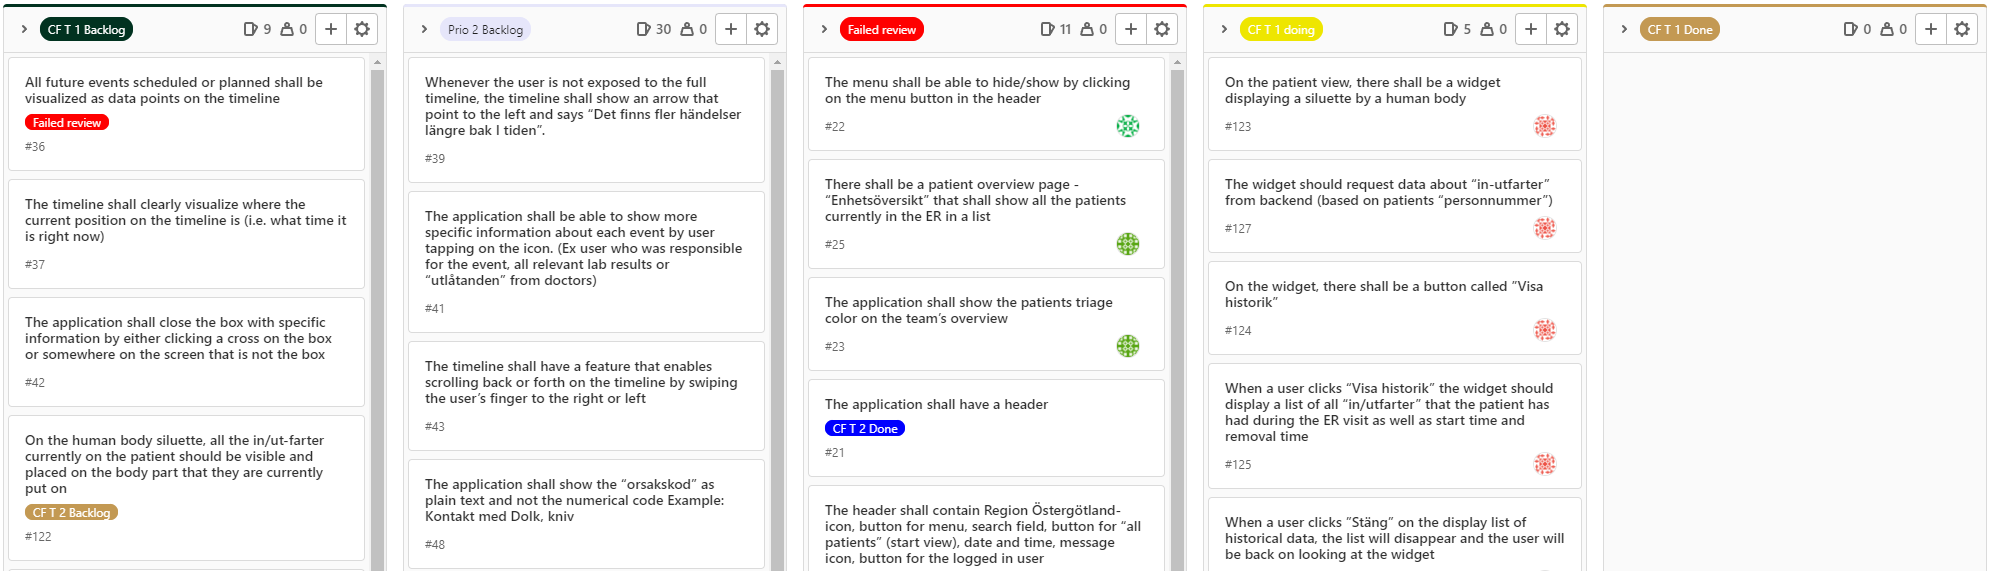
\includegraphics[width=1 \linewidth]{figures/Gitlab board.PNG}
     \caption{GitLab Board}
     %\label{appendix: gitlabboard}
\end{figure}




\clearpage

%----------------------------------------------------------------------------------------
%	Appendix
%----------------------------------------------------------------------------------------
% \newpage
\appendix

\section{Development process}
\label{sec:dev-process-appendix}
 \begin{figure}[h!]
     \centering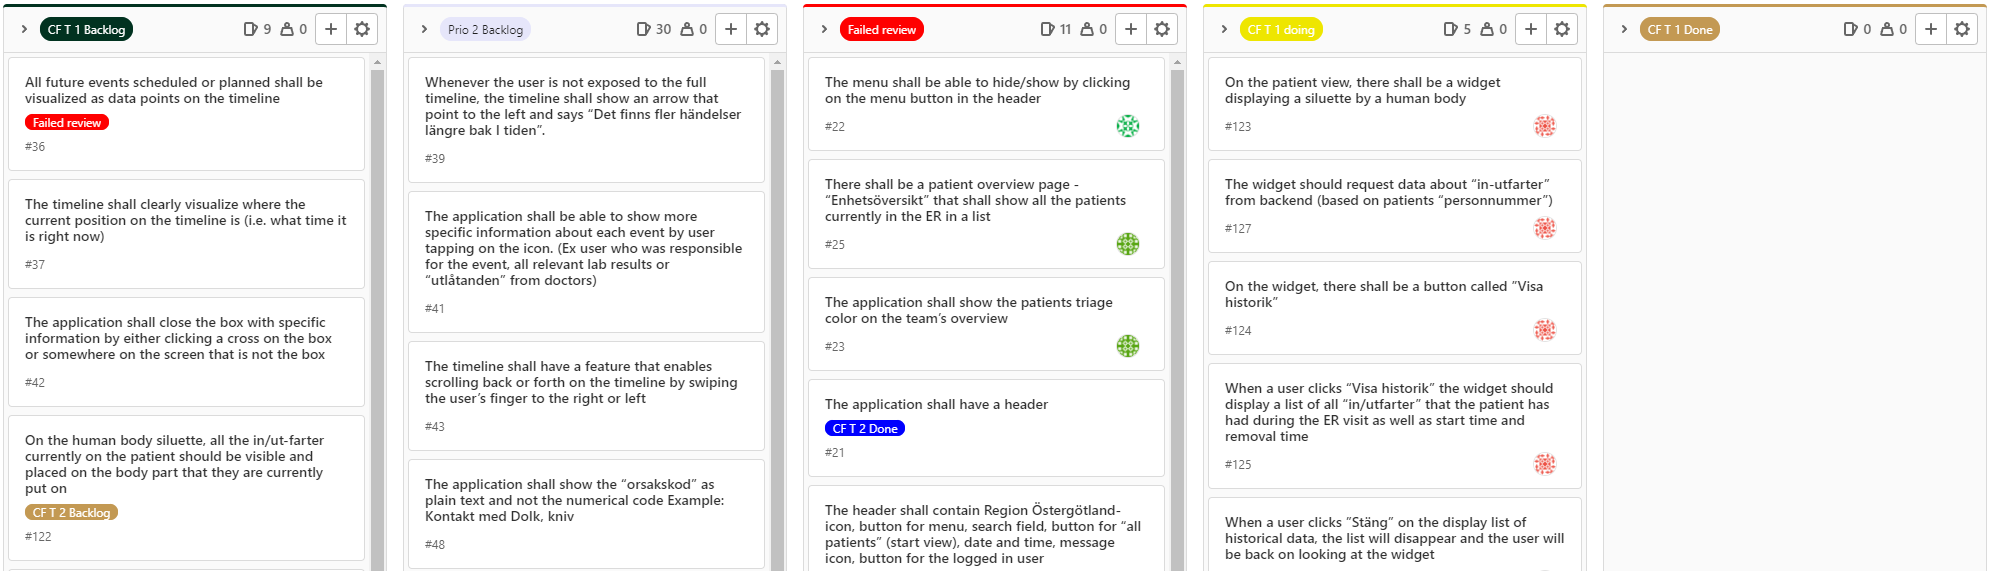
\includegraphics[width=1 \linewidth]{figures/Gitlab board.PNG}
     \caption{GitLab Board}
     %\label{appendix: gitlabboard}
\end{figure}



%----------------------------------------------------------------------------------------
%	Bibliography
%----------------------------------------------------------------------------------------
\clearpage
%References (add if needed)
% \bibliography{bibliography/sample}{}
% \bibliographystyle{plain}

\end{document}